

A protostellar disk is composed mostly of gas, accounting for approximately 99\% of its mass, with the remaining 1\% consisting of dust. Although dust accounts for a small fraction of the mass, it plays a vital role in the evolution of the disk and the formation of planets, providing the raw material that eventually forms terrestrial planets and the cores of giant planets \citep{Williams, Birnstiel2016}.

\subsection{Dust Evolution and Grain Growth}





% The dust in protostellar disks originates from the ISM and is typically sub-micron in size \citep{Williams}.

Dust grain growth, or dust coagulation, is an early stage of planet formation in which grain-grain collisions can cause dust particles to stick together and form larger particles. During this phase, the grains begin as sub-micron-sized particles and can grow, eventually leading to the formation of $>$ km-sized planetesimals \citep{Birnstiel2016}. It is thought that this earliest stage of planet formation may be occurring as early as the Class I phase \citep{Dom2020}. 

During grain-grain collisions, the grains do not always stick together to become larger. The grains can also bounce off each other, leaving their sizes mostly unchanged, or they can fragment and produce smaller grains, either with or without mass transfer. The result of the collision depends on the velocity and relative sizes of the particles colliding \citep{Testi}.



\subsection{Dust Distribution and Disk Structure}

As grains change in size, their interactions with the surrounding gas change, altering how they are transported both vertically and radially within the disk \citep{Andrews}. Small grains ($\sim$0.1 \micronNS) are well coupled to the gas due to drag forces and are expected to move with it.  As the grains grow in size, however, the drag forces can cause a headwind that removes angular momentum from the dust and effectively decouples the dust motion from the gas.  These decoupled grains tend to settle vertically to the midplane and move radially inward \citep{Dullemond2004, Barri2005, Birnstiel2016}.


% This sentence is too long
% Small grains ($\sim$0.1 \micronNS) have a large surface-to-mass ratio, are well coupled with the gas, and experience a strong drag force as their motion follows the gas \citep{Dullemond2004, Birnstiel2016}.




% % medium sized objects feel drag
% As the grains grow, their surface-to-mass ratio decreases, and their motion decouples from the gas, also creating a downward drag force \citep{Williams}. 






% Because the dust grains do not respond to the gas pressure, they orbit faster than the gas and experience a drag force. Thus, the drag force decreases the angular momentum of the grains, causing them to drift radially inward toward the centre of the disk \citep{Krumholz}. 


%very large objects do not feel drag. This is the meter-size barrier problem, where meter-sized grains feel the most drag and spiral into the star faster than they can grow and decouple from the gas. 
% Dust grains that are very large (mm to cm) allow particles to decouple from the gas \citep{Birnstiel2016}. 






At distances further from the central star, the gravitational influence of the star is weaker, allowing grains to move off of the midplane. As a result, the disk's scale height increases with distance from the centre, causing a flared disk. As these grain-grain collisions, gravitational effects and turbulent mixing all work together, larger grains typically reside near the midplane, while smaller grains are higher up. Figure \ref{fig: dust-grain-growth-schematic} illustrates these processes and the resulting dust distribution.




\begin{figure}[htbp]
  \centering
  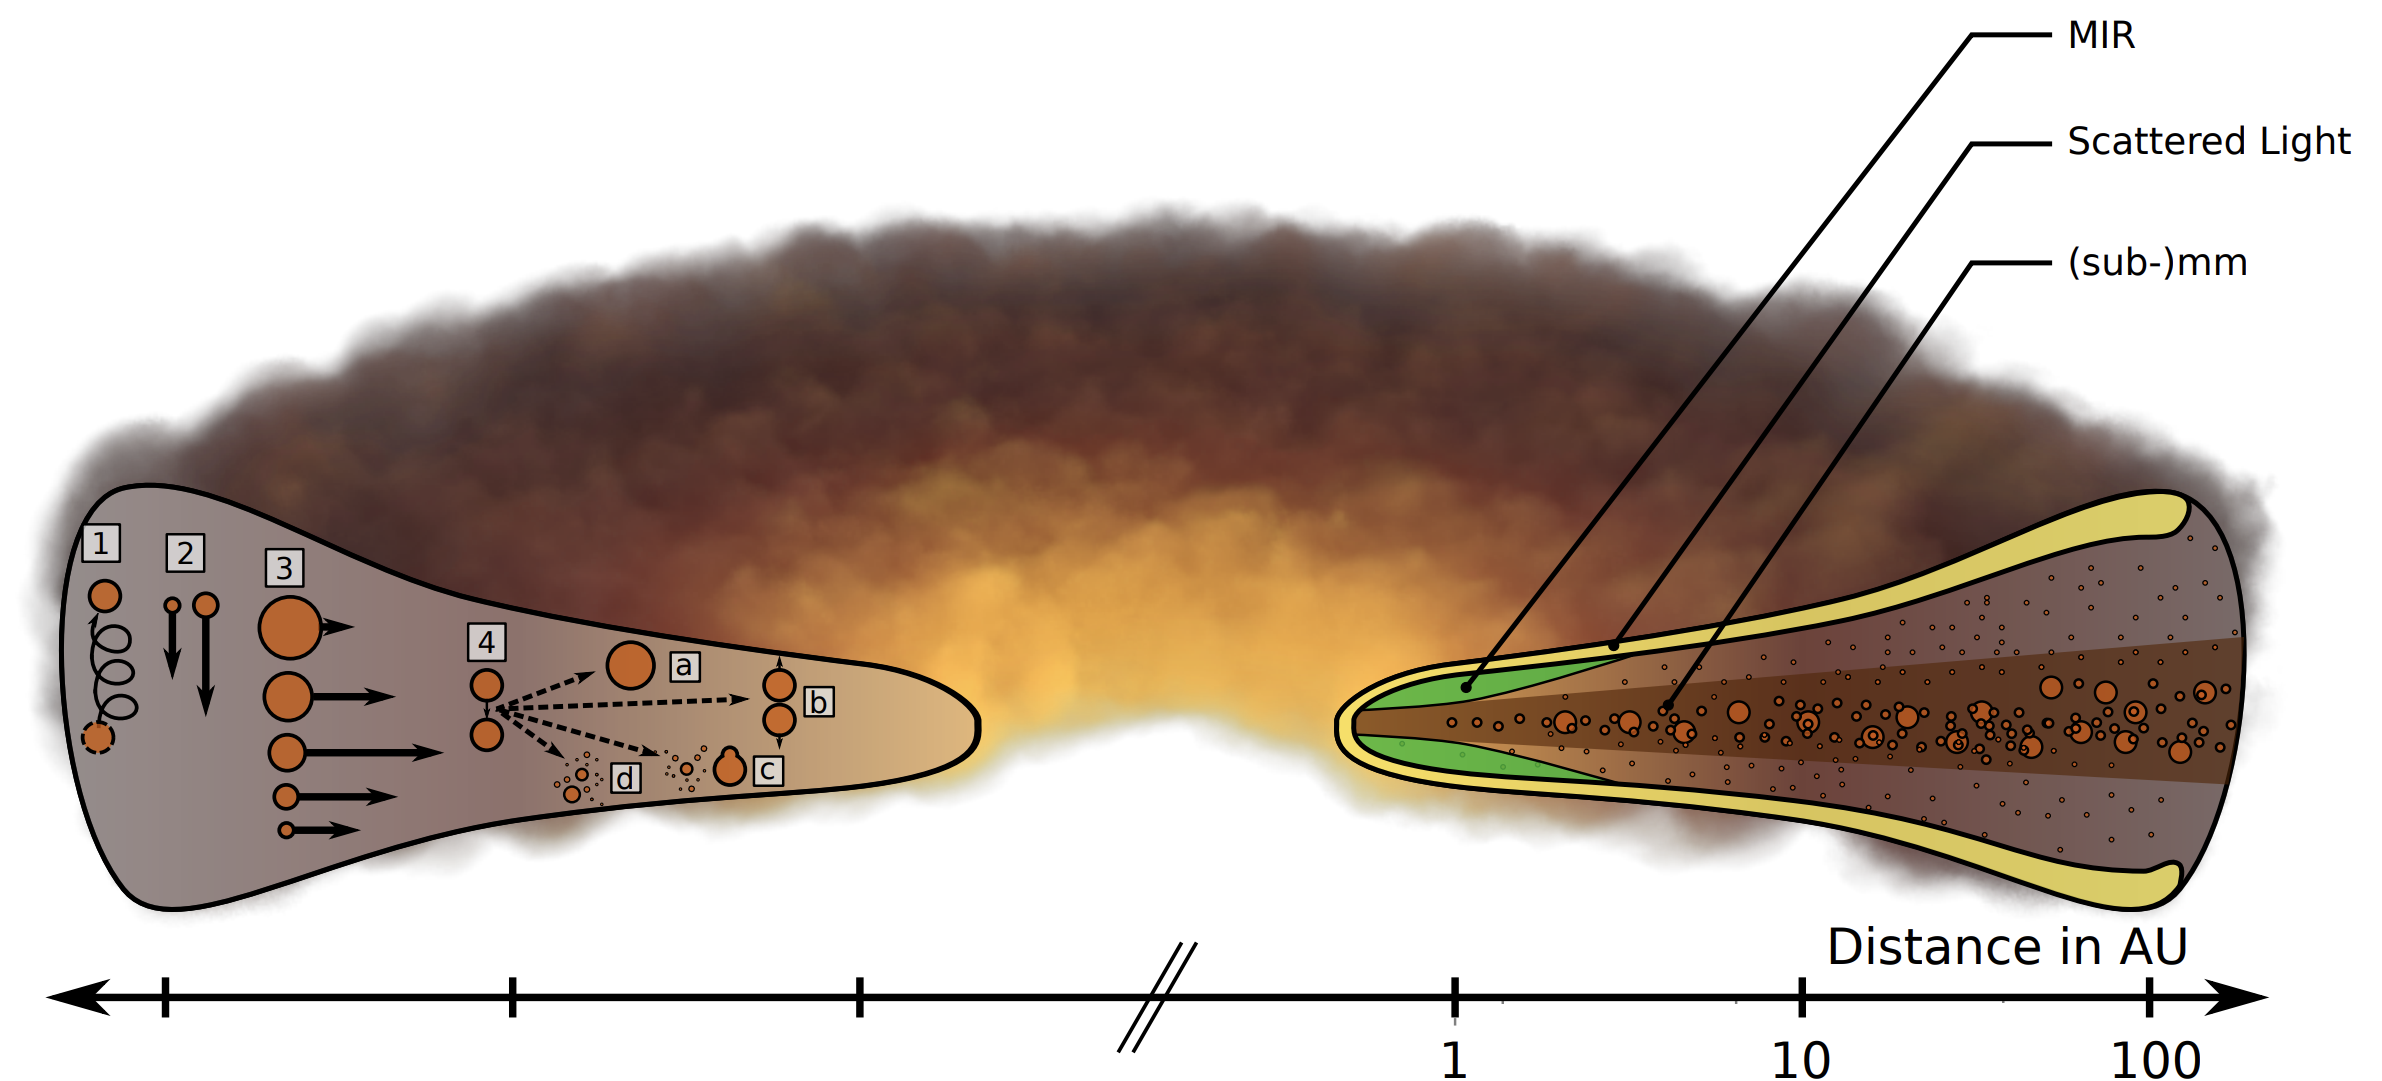
\includegraphics[width=0.9\textwidth]{WRITEUP_AND_IMAGES/IMAGES/WRITEUP/NOTMINE/Testi_short.png}
  \caption[Schematic of the structure and grain evolution process.]{Schematic of the structure and grain evolution process for a protostellar disk. Numbers refer to grain transport and collision processes: (1) turbulent mixing (radial or vertical), (2) vertical settling, (3) radial drift, and (4) grain collision outcomes, including (a) sticking, (b) bouncing, (c) fragmentation with mass transfer, and d) fragmentation. Different arrow lengths show different velocities of the grains. Image from \cite{Testi}, reproduced with permission. }
  \label{fig: dust-grain-growth-schematic}
\end{figure}








%%%%%%%%%%%%%%%%%%%%%%%%%%%%%%%%%%%%%%%%%%%%%%%%%%%
%%%%%%%%%%%%%%%%%%%%%%%%%%%%%%%%%%%%%%%%%%%%%%%%%%%
\subsection{Effects of Grain Size on Dust Opacity}
\label{sec: intro_dust_grainsize}


% Dust grains control how opaque or transparent (opacity) the disk is since gas doesn't as much. 
Dust grains dominate the opacity in protostellar disks, controlling how radiation interacts with the disk through absorption and scattering \citep{Williams}. At (sub)millimetre wavelengths, the continuum emission from disks is dominated by thermal emission from the dust. 


The efficiency by which dust grains absorb and emit light depends on their absorption opacity. The opacity depends on several properties of the dust, including its composition, shape and size relative to the observing wavelength \citep{Testi, Kataoka_2015}. Figure \ref{fig: kappa_vs_lambda} shows the dependence of the absorption and scattering opacities on wavelength for two grain sizes:  1\micron and 100 \micronNS. For the smaller grains, absorption dominates over scattering across the majority of the wavelengths shown. For the larger grains, scattering becomes much more important, with the scattering and absorption opacities becoming comparable at shorter wavelengths and scattering dominating over a range of wavelengths. This is discussed more in Chapter \ref{sec: ch5_opticalproperties}.





% ----------------------------------------------
\begin{figure}[htbp]
  \centering
  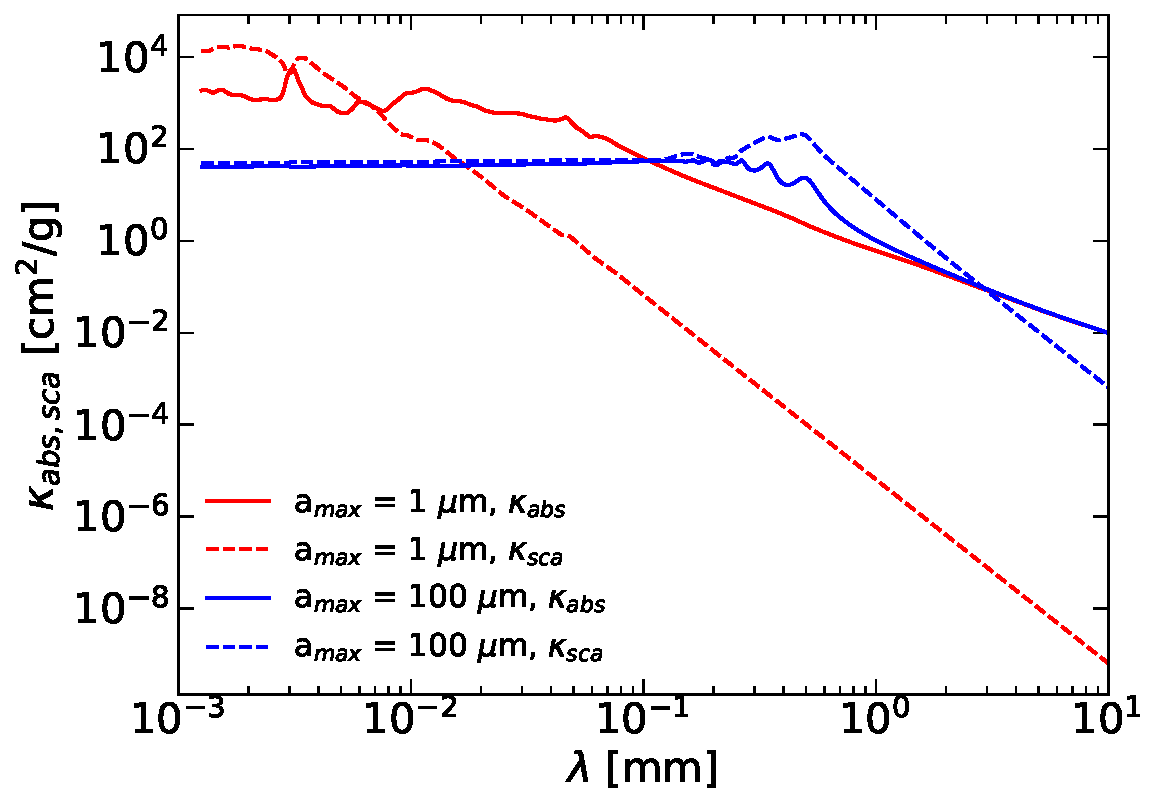
\includegraphics[width=0.75\textwidth]{WRITEUP_AND_IMAGES/IMAGES/WRITEUP/DustModels/Kataoka2015Fig1.pdf}
  \caption[Absorption and scattering mass opacities.]{Absorption and effective scattering mass opacities as a function of observing wavelength for grain sizes of 1\micron and 100 \micronNS. Replication based on Figure 1 from \cite{Kataoka_2015}.}
  \label{fig: kappa_vs_lambda}
\end{figure}
% Recreation of Figure 1 from \cite{Kataoka_2015}. 
% ----------------------------------------------

